\chapter{Background: GDPR and the Semantic Web}
\label{chapter:background}

This chapter presents the necessary background information related to understanding the research presented in this thesis. In particular, it presents a short introduction to the General Data Protection Regulation (GDPR) in \autoref{sec:background:GDPR} and to the semantic web in \autoref{sec:background:semweb}. The information only represents a summary of the topic and is accompanied with links in the footnotes which further information.

\section{General Data Protection Regulation (GDPR)}\label{sec:background:GDPR}
The General Data Protection Regulation (GDPR) \cite{noauthor_regulation_2016} is the current data protection law applicable within the European Union (EU) and the European Economic Area (EEA) and regulates the use and processing of personal data. 
It supersedes its predecessor - the Data Protection Directive (DPD) \cite{noauthor_directive_1995} - and provides greater requirements and transparency for its compliance, as well as a potentially large and significant amount of fines if organisations are found to have violated its obligations.
A significant aspect of the GDPR are its principles and rights which are intended to afford the individual greater privacy and control regarding the use of their personal data.

By virtue of it being a regulation as opposed to a directive, it is considered enforceable law with local and national implementations acting in conjunction with it rather than replacing it.
The GDPR has attracted global attention and scrutiny due to its requirements for compliance and potential fines, as well as for providing rights which enhance privacy.
It has directly been influential in other privacy laws across the laws, with the California Consumer Protection Act (CCPA) being a significant law that follows many of its provisions and requirements \cite{marini_gdpr_2018}.

\subsection{Terminology}
The legal terminology utilised in GDPR is intended to clarify the roles, actions, and concepts upon which the law specifies obligations.
The definition of \textit{\textbf{personal data}} (Article 4-1) is based on the linking, association, or relevance of any information with an individual - and represents a significant change from its predecessor as well from other laws which rely upon the concept of Personally Identifiable Information (PII). The individual the personal data relates to is termed as the \textit{\textbf{Data Subject}} (Article 4-1), which is again a distinct term from other relevant laws where the term \textit{individual} or \textit{PII Principal} are used.

GDPR regulates \textit{\textbf{processing}} of personal data (Article 4-1) which is defined as any action over or utilising personal data, with its definition providing a range of activities - ``collection, recording, organisation, structuring, storage, adaptation or alteration, retrieval, consultation, use, disclosure by transmission, dissemination or otherwise making available, alignment or combination, restriction, erasure or destruction;'' \cite{noauthor_regulation_2016}.

A \textit{\textbf{Controller}} is defined (Article 4-7) as the entity or organisation that determines the \textit{\textbf{purpose}} and means of processing of personal data. As such, the controller is the primary organisation in the context of the GDPR and is the subject of more obligations given its role in the processing of personal data. One or more controllers can act together to determine the purpose and carry out the processing, in which case they are defined as \textit{\textbf{Joint-Controllers}} (Article 26).

A \textit{\textbf{Processor}} is defined (Article 4-8) as an entity which processes the personal data on specified instructions of the controller (Article 28) and is not allowed to deviate from the instructions or utilise the personal data for other purposes. A processor is also referred to as \textit{contractor} in some contexts. A processor may appoint other \textit{sub-processors} in order to carry out processing, where the sub-processors are requried to follow the same obligations as the processor.

A \textit{\textbf{Data Protection Officer (DPO)}} is defined (Article 37) as an individual appointed by the controller or processor to oversee the compliance and processing of personal data, monitor internal processors, and collaborate with supervisory authorities as required.

A \textit{\textbf{Regulatory or Supervisory Authority or Data Protection Commission}} is a governmental organisation with the responsibility to evaluate and enforce GDPR compliance. These bodies are established within the context of national or federal governments and have jurisdiction over their appointed regions. The GDPR lays out the responsibilities of such bodies and provides avenues for their co-operation across jurisdictions (Article 56, 60, 62).

GDPR provides several \textbf{\textit{rights}} to the data subject (Chapter 3) which are obligated to be provided by controller(s). Such rights are mandatory under the GDPR and therefore their implementation, provision, and exercising carries with it several requirements towards compliance.

\subsubsection{PRIPARE}
PRIPARE\footnote{\url{http://pripareproject.eu/}} (PReparing Industry to Privacy-by-design by supporting its Application in REsearch) is an European research project that aimed to provide a set of documents regarding privacy engineering by covering activities such as privacy risk management, requirement analysis, design strategies, maintenance and compliance. To this end, it published the PRIPARE methodology handbook \cite{noauthor_pripare-methodology-handbook-final-feb-24-2016.pdf_nodate} providing guidelines for privacy and security by design. The handbook incorporates information based on a draft of GDPR\footnote{\url{The handbook was published in 2015, and incorporated known information about the GDPR up to that point in time.}} It provides foundational methodologies and reference models for carrying out privacy analysis, designing and implementing privacy enhancing systems, with templates for impact assessments and conformance. 

\subsubsection{STAR \& STAR II}
STAR\footnote{\url{https://projectstareu.wordpress.com/}} (Support Training Activities on the data protection Reform) is an European project that had the aim to provide materials to support training of DPAs and DPOs for the GDPR. To this end, it has created and published its resources consisting of training materials in an open and publicly accessible form\footnote{\url{http://www.project-star.eu/training-materials}}. The project has also produced a handbook for assisting stakeholders in understanding the GDPR and preparing for its compliance. The project also provides an evaluation questionnaire and compliance checklist \cite{noauthor_gdpr_2019-1}consisting of a list of questions and criterion to assess preparedness with the requirements of the GDPR. 

The resources published by the STAR projects provide documentation regarding GDPR compliance that is adopted by organisations and regulatory authorities. As such, it acts as a source of information about GDPR in the requirements gathering phase associated with information representation and evaluation of compliance.

\section{Semantic Web Technologies}\label{sec:background:semweb}
% This section provides background information on the semantic web. It introduces the semantic web standards of RDF, RDFS, OWL, SPARQL, and SHACL.
% Through these concepts, the application of linked data towards information management is described.

The term `\textit{Semantic Web}' refers to the extension of the world wide web with machine-readable and interoperable metadata to enable encoding of semantics with the data.
This is achieved through the use of standards developed by the World Wide Web Consortium (W3C) which promotes common data formats for interoperability and data exchange protocols using the infrastructure of the web.
The \autoref{fig:bg:semantic-web-stack} shows the `\textit{Semantic Web Stack}' which presents the architecture and relationship of the different components within the semantic web.
\begin{figure}[htbp]
    \centering
    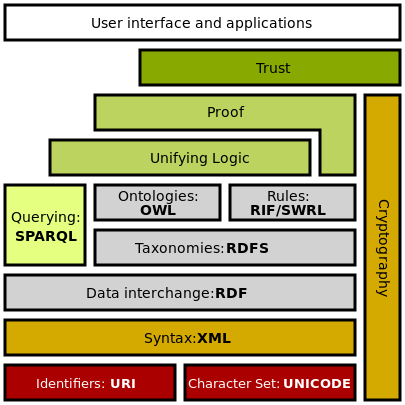
\includegraphics[width=0.75\linewidth]{img/Semantic_web_stack.png}
    \caption{Semantic Web Stack}
    \label{fig:bg:semantic-web-stack}
\end{figure}

\subsection{RDF, RDFS, and OWL}

\subsubsection{Resource Description Framework (RDF)}
The representation of semantics starts with the specification of facts or `knowledge' using RDF\footnote{\url{https://www.w3.org/TR/rdf11-concepts/}}, which provides representation of information in the form of triples whose collective expression can be visualised as a graph.
The RDF triples are serialised using syntax languages such as XML\footnote{\url{https://www.w3.org/TR/rdf-syntax-grammar/}}, or the more human-readable Turtle\footnote{\url{https://www.w3.org/TR/turtle/}}, or the web friendly JSON-LD\footnote{\url{https://www.w3.org/TR/json-ld/}}.
RDF triples utilise the same identifier system as the world wide web and are specified using IRIs\footnote{\url{https://tools.ietf.org/html/rfc3987}} - which are a generalised form of URIs which itself are a generalised form of URLs\footnote{\url{https://www.w3.org/TR/uri-clarification/}}.
A database storing RDF is called a triple-store and enables the creation of graphs of RDF datasets and provides an interface for querying it.

A RDF triple consists of a subject, an object, and a predicate - where the predicate describes the relationship from the subject to the object. An example of RDF triple specified using the Turtle language to indicate the chapter number of an entity is expressed as -\\ \-\hspace{5mm}\mintinline{turtle}{<http://example.com/ch2> foaf:name "Background"@en .}\\
The subject in this triple is the IRI \mintinline{turtle}{<http://example.com/ch2>} representing a resource, with the predicate \mintinline{turtle}{foaf:name} representing the relationship of associating a name as indicated by the string in the object field \mintinline{turtle}{"Background"@en} with \texttt{@en} specifying it is in the English language. 

The subject is written in shorthand notation indicating it starts with the same IRI as the data file it is described in. A complete IRI is often long to write and is usually written using shorthand prefixes intended for human-readability.
The predicate is a \textit{property} provided by an external ontology called `Friend of a Friend' (FOAF\footnote{\url{http://xmlns.com/foaf/spec/}}), which is referenced by its prefix \texttt{foaf} as shorthand for its entire IRI.
The object is a string in this case, but could itself be another RDF triple or resource - in which case it would be specified as an IRI.

\subsubsection{RDF Schema (RDFS)}
RDFS provides concepts for expressing classes, properties, and datatypes in order to represent schemas using RDF. It also provides commonly required relationships such as specifying labels of a resource, indicating a related resource, or specifying the domain and range of properties. The example in the code below expands upon the triple described in RDF to express chapter as a class with its number as a property, and specifies human-readable labels for each resource.
\begin{minted}{turtle}
@prefix foaf: <http://xmlns.com/foaf/0.1/> .
@prefix : <http://example.com/> .
:Ch2 rdf:type :Chapter ; foaf:name "Background"@en ; :chnum 2^^xsd:integer .
:Chapter rdf:type rdfs:Class ; rdfs:label "Chapter"@en .
:chnum a rdfs:Property ; rdfs:label "number"@en ; rdfs:range xsd:integer .
\end{minted}

\subsubsection{Web Ontology Language (OWL)}
While RDFS enables expression of hierarchies, more formal representations of knowledge modelling and logic require additional constructs. These can be represented using OWL\footnote{\url{https://www.w3.org/TR/owl2-overview/}} in the form of an ontology consisting of a set of `individuals' (also called classes) and a set of `property assertions' which relate individuals to each other.
An ontology may also consist of a set of axioms which place constraints on sets of individuals and the types of relationships permitted between them. These axioms provide semantics which can be used to infer additional information using semantic reasoners based on the information explicitly provided.
Knowledge expressed using OWL can be (and generally is) expressed using RDF, which makes it possible to encode and store ontologies in the form of RDF data.

\subsection{SPARQL Protocol and RDF Query Language (SPARQL)}
SPARQL\footnote{\url{https://www.w3.org/TR/sparql11-query/}} is a query language for retrieving data expressed using the semantics provided by RDF.
SPARQL queries information following the RDF specification, and thus specifies its queries to act on data expressed as a set of `subject-predicate-object' triples.
SPARQL queries can also retrieve information from traditional (SQL) databases which store data in non-RDF form through the use of mapping\footnote{\url{https://www.w3.org/2008/07/MappingRules/StemMapping}}, which permits its semantics to be applied across a large variety of existing data stores.

A SPARQL endpoint is an interface provided by a triple-store to provide access and querying over the data stored within it. Such endpoints can be exposed over the web to provide querying capabilities using the internet, with DBPedia\footnote{\url{http://dbpedia.org/sparql}} - a semantic web representation of Wikipedia - providing a well-known example.

\subsection{Shapes Constraint Language (SHACL)}
SHACL\footnote{\url{http://dbpedia.org/sparql}} is a specification language for expressing constraints that validate RDF data. The input over which SHACL constraints are validated is called the \textit{data graph}.
Constraints in SHACL are called `shapes' based on the notion of checking if data \textit{fits a shape}, and therefore the set of constraints being validated are called as the \textit{shapes graph}.
SHACL constraints are themselves also expressed in RDF which makes it possible to serialise them as a data graph and perform querying over it.

The output of the validation process is a conformance report which uses a validation report vocabulary provided by SHACL and indicates the \textit{failing validations} and the status of validation of a whole. A \textit{conformance report} is a boolean indication of whether the any of given set of validations have failed, or conversely whether all validations have passed.

SHACL-core refers to the defined features within the SHACL standard specification. Extensions have been developed which provide additional features in the expression and validation of constraints using the features of SHACL-core. Amongst these, SHACL-SPARQL provides the use of SPARQL queries to retrieve failing data, and is mentioned within the SHACL specification.
SHACL validations are performed using a `validator' which is an implementation and interpretation of the SHACL standard and provides at least the validation features described in SHACL-core.

\subsection{Standardised Ontologies}
\subsubsection{Provenance Ontology (PROV-O)}
PROV-O\footnote{\url{https://www.w3.org/TR/prov-o/}} is a standardised ontological representation of the PROV Data Model\footnote{\url{https://www.w3.org/TR/prov-dm/}} (PROV-DM) which is the W3C standard for representing provenance information using the semantics provided by RDF and OWL.
PROV-O provides a set of classes, properties, and restrictions that can be used to represent and interchange provenance information within different contexts.
It can also be specialised to create new classes and properties to model provenance information for different applications and domains.

\subsubsection{Open Digital Rights Language (ODRL)}
ODRL\footnote{\url{https://www.w3.org/TR/odrl-model/}} is a policy expression language that provides an information model, vocabulary, and encoding mechanisms for representing statements about the usage of content and services in the form of policies. The ODRL Information Model describes the underlying concepts, entities, and relationships that form the foundational basis for the semantics of the ODRL policies.
Policies are used to represent permitted and prohibited actions over one or more assets and can also contain obligations required to be met by stakeholders.
Policies can also specify constraints, such as temporal or spatial, and duties which are required to be carried out.
ODRL conformance is based on evaluating whether a given information representing an use-case or context satisfies all the expressions described in a given policy.